
An overview of \toolName\ is depicted in Fig.~\ref{fig:overview}.
\toolName\ takes as input the models for the robots (\circled{1}) and of the environment in which they are deployed (\circled{2}) and the mission each robot should achieve (\circled{3}).
Both the models of the robots and their environment may be partial since there can be uncertainty about information contained in these models.
\toolName\ uses the model of the environment and the robots to compute plans that allows to achieve missions using an appropriate planner.
The implemented planner is able to compute plans that definitely ensure the mission satisfaction, i.e., definitive plans  (\circled{4}), and plans that may ensure property satisfaction since they depend on some partial knowledge present in the models of the robots and the environment  (\circled{5}).
More precisely, a \emph{definitive plan} is a sequence of actions that ensure the satisfaction of the local mission for each robot. 
A \emph{possible plan} is a sequence of actions that may satisfy the local mission due to some unknown information about the model of the robots or the environment in which they are deployed. 
If \toolName\ not able to find neither a definitive nor a possible plan a message is sent to the user.
Otherwise an appropriate component is used to choose between definitive and a possible plans (if both are present) or simply chooses the possible plan if no definitive plan is present.
Definitive plans are not present when the only way to satisfy the local mission is based on some unknown information about the model of the robots or the environment in which they are deployed. 
\toolName\ then executes the selected plan (\circled{6}).
As robots perform plans information about uncertain parts of the model is detected.
\toolName\ updates the   models with the detected information (\circled{7}).
If \toolName\  detects that a plan not any more executable, the planner is re-executed (\circled{8}).
In the following we provide some additional information about the inputs processed  by \toolName, the planning algorithm, the selection between definitive and possible plans and how models are updated when information about uncertain parts is detected.


\begin{figure}[h]
\begin{center}
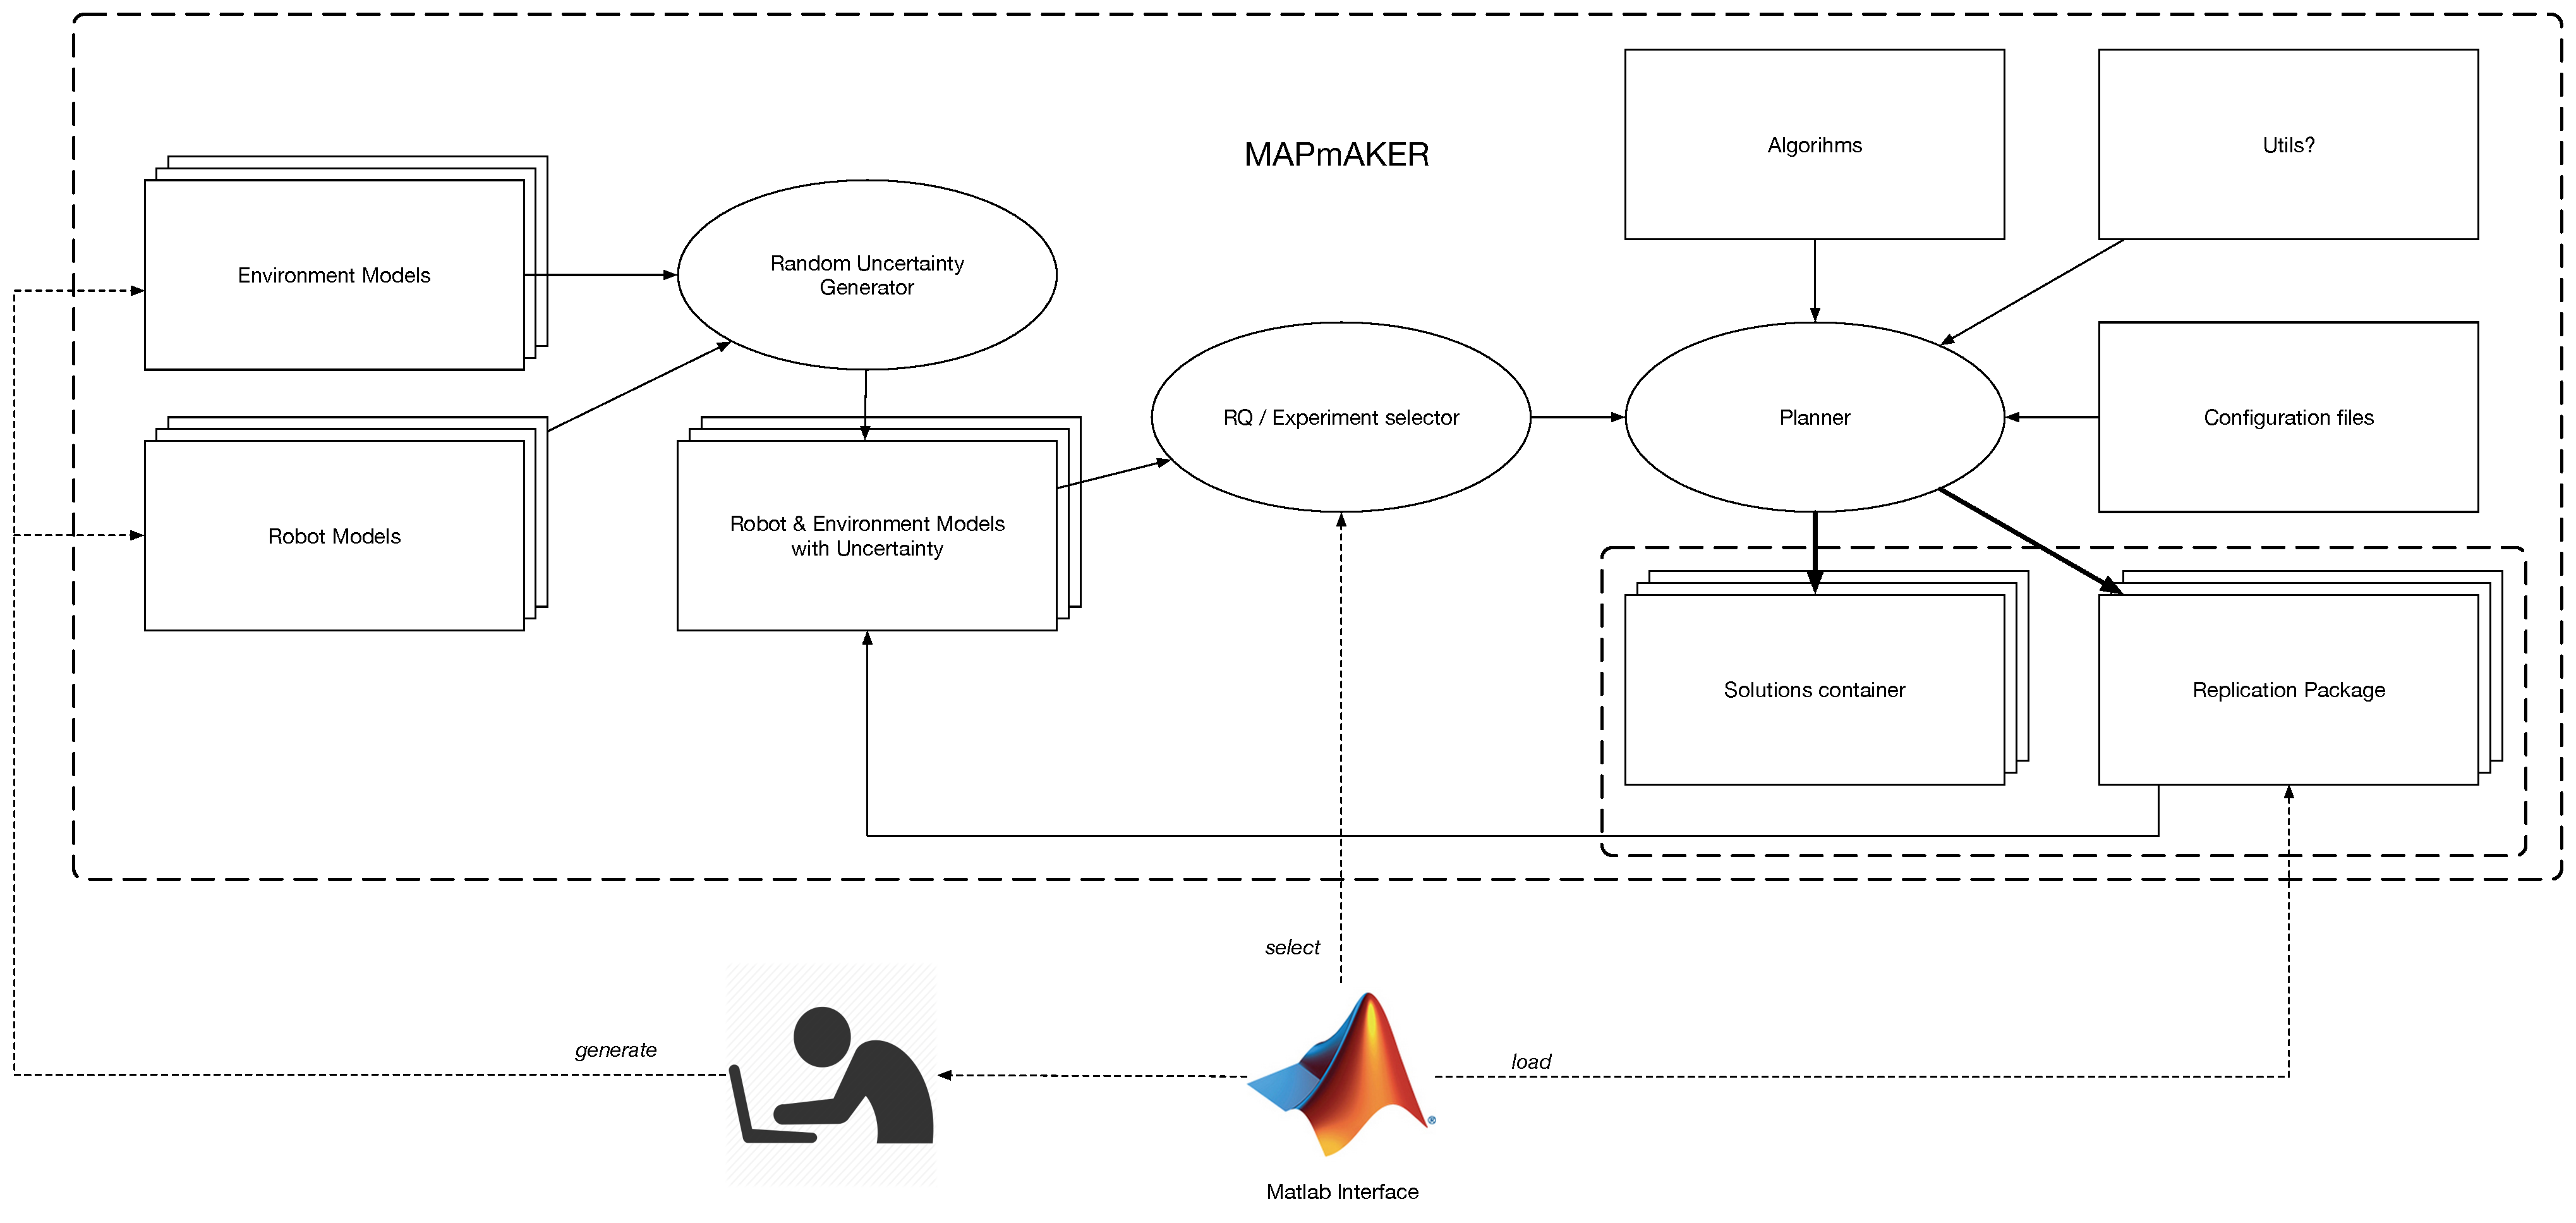
\includegraphics[width=1\linewidth]{Figures/MAPmAKER.pdf}
\caption{Overview on  MAPmAKER.}
\label{fig:overview}
\end{center}
\end{figure}


\textbf{Models of the robots and the environment}. 
The models of the robots and their environments are provided using some form of transition system that allows the specification of uncertain parts.
Specifically, the proposed models supports the specification of
%\textbf{Uncertainties supported by \toolName}.
\begin{itemize}
\item  \emph{Partial knowledge about the actions execution.} 
The transition between two of the cells that conform the grid map of the environment can be:
always possible, always not possible (i.e. a wall), not known (i.e. a door between two rooms that can be open or closed).
\item \emph{Unknown service provisioning.} 
In the dynamic environments studied for this work whether a service is provided or not in a specific location could be unknown. 
In order to achieve the mission with the minimum number of actions performed, \toolName~ is able to compute a plan that tries to reach an uncertain service.
Thus, \toolName~ computes a \emph{possible plan}.
\item \emph{Unknown meeting capabilities.} 
As stated before, robots can meet and synchronize in certain locations.
There they can perform a mission, as exchanging a load, in a collaborative fashion.
In this case, two or more robots that are part of the same subset part of the whole team can compute a plan whose goal is to meet in an uncertain synchronization point.
Thus, \toolName computes a \emph{possible plan}.
\end{itemize}

The model of each robot contains information regarding its initial position, the number of services that the robot must perform and their location and the locations where the modeled robot has to synchronize with another one.  
The model of the environment represents its map and defines the allowance of transitions between the cells that compound the model (i.e. walls). 
This two models must be manually defined but can be reused for an infinite number of experiments.





\textbf{Mission specification.}
Each robot is able to perform a complex mission, which is specified using an LTL formula.
These formula specified how the services must be provided by robots.
For example, the mission for robot $r_1$ may require that  periodically robot $r_1$ loads debris on $r_2$.
Note that, in order to allow robot $r_1$ to achieve its mission it is necessary for robots $r_1$ and $r_2$ to synchronize.





\textbf{Planning.} 
The \emph{Planner}  uses the models of the robot(s) and the environment in order to compute plans that allows satisfying the missions of the robots.




\textbf{Choosing between definitive and possible plans.}
The tool always try to reach the goal performing the lower number of actions.

\textbf{Detection of uncertain information.}
Whenever a robot approaches to an location with uncertain information, it detects if this transition, service, or meeting capability is detected to be firable, provided, and possible, respectively.
The robot then updates the information concerning to this location, setting it yo ``true" or ``false".
This information is shared with the rest of the team so it can be take into account for further planning.






